\section{Measurement}
\begin{figure}[htbp]
    \centering
    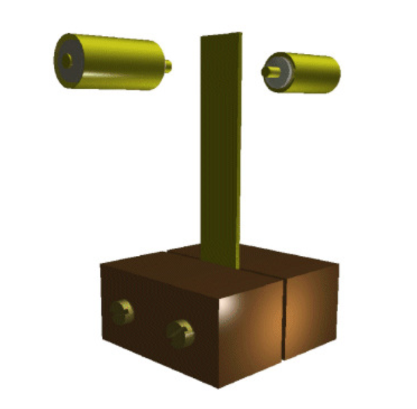
\includegraphics[width=.6\linewidth]{./Assets/setup.png}
    \caption{The setup of a \quotemention{vibrating reed} experiment. Taken from \autocite[1]{fp75}.}
    \label{fig:setup}
\end{figure}
The subject of this experiment is the so-called \quotedef{vibrating reed,} pictured in \autoref{fig:setup}.
It consists of a metal plate which

% A
% Nehmen Sie die Resonanzkurven für die drei Frequenzen ν0, ν1 und ν2 auf.

% B
% Temperaturabhangigkeit der Resonanzfrequenz

% I
% Sie nehmen eine komplette Resonanzkurve fur jede eingestellte Temperatur.

% II
% Mit dieser Methode kann man die Temperaturabhängigkeit viel schneller messen und ohne Nachtmessung auskommen. Man benutzt dabei das A cos ϕ-Signal des Lock-In-Verstärkers. Zunächst stellt man die Spannung im Peltier-Element entsprechend der Temper


% (
% • Was wollen wir im Abschnitt A und B messen?
% • Versuchsplanung: Wie wollen Sie die Resonanzfrequenzen im Abschnitt A finden?
% • Was sind Vor- und Nachteile der beiden Methoden für die Messung im Abschnitt B?
% )